%\documentclass[preprint]{sigproc}
\documentclass{acm_proc_article-sp}

% The following \documentclass options may be useful:
%
% 10pt          To set in 10-point type instead of 9-point.
% 11pt          To set in 11-point type instead of 9-point.
% authoryear    To obtain author/year citation style instead of numeric.

\setlength{\textfloatsep}{5pt}

\usepackage{flushend}
\usepackage{graphicx}
\usepackage{verbatim}
\usepackage{url}
\usepackage{alltt}
\renewcommand{\ttdefault}{txtt}

\usepackage{amsmath}
\usepackage{dsfont}
\usepackage{mathtools}
\everymath{\displaystyle}
\usepackage{xspace}

\newcommand{\CEU}{\textsc{C\'{e}u}\xspace}
\newcommand{\code}[1] {{\small{\texttt{#1}}}}
\newcommand{\DOFIN}{\code{do-finally}\xspace}
\newcommand{\FIN}{\code{finally}\xspace}

\newcommand{\ST}{\1\xrightarrow[~n~]{}\1}
\newcommand{\BT}{\xRightarrow[(i,E)]{}}
\newcommand{\LL}{\langle}
\newcommand{\RR}{\rangle}
\newcommand{\DS}{\displaystyle}
\newcommand{\rr}[1] {{\textbf{\scriptsize{#1}}}}


\newcommand{\1}{\;}
\newcommand{\2}{\;\;}
\newcommand{\3}{\;\;\;}
\newcommand{\5}{\;\;\;\;\;}
\newcommand{\ten}{\5\5}
\newcommand{\twenty}{\ten\ten}

\newenvironment{itemize*}%
  {\begin{itemize}%
    \setlength{\itemsep}{0pt}%
    \setlength{\parskip}{0pt}}%
  {\end{itemize}}

\usepackage{enumitem}
\setlist{nolistsep}

\usepackage{color}
\definecolor{light}{gray}{0.87}
\definecolor{dark}{gray}{0.30}
%\definecolor{light}{rgb}{.90,.90,.90}
\definecolor{darkgreen}{rgb}{0,.50,0}
\definecolor{darkblue}{rgb}{0,0,.50}
\definecolor{darkred}{rgb}{.50,0,0}
\definecolor{darkpur}{rgb}{.50,0,.50}

\usepackage{listings}
%\usepackage{textcomp}
\lstset{
%columns=fullflexible,
%basicstyle=\ttfamily,
escapeinside={||},
mathescape=true,
    language=C, % choose the language of the code
    basicstyle=\fontfamily{pcr}\selectfont\scriptsize\color{black},
    keywordstyle=\color{black}\bfseries, % style for keywords
    numbers=none, % where to put the line-numbers
    numberstyle=\tiny, % the size of the fonts that are used for the line-numbers
    backgroundcolor=\color{light},
    showspaces=false, % show spaces adding particular underscores
    showstringspaces=false, % underline spaces within strings
    showtabs=false, % show tabs within strings adding particular underscores
    %frame=single, % adds a frame around the code
    tabsize=2, % sets default tabsize to 2 spaces
    %rulesepcolor=\color{gray}
    captionpos=t, % sets the caption-position to bottom
    breaklines=false, % sets automatic line breaking
    %breakatwhitespace=false,
    numbersep=2em,
    emph={par,or,hor,do,end,loop,await,emit,input,event,call,with,command,%
          var,and,then,else,C,return,pure,deterministic,nohold,finalize,%
          each, abort, when, signal},
    emphstyle={\bfseries},
    commentstyle=\color{dark}\scriptsize,
    %xleftmargin=20pt,
    %xrightmargin=20pt,
    framesep=20pt,
    %upquote=true,
    %aboveskip={1.5\baselineskip},
}

\begin{document}

\title {
    Reconciling Control and Dataflow Reactivity in Embedded Systems
}

\numberofauthors{1}
\author{
    \alignauthor
    Francisco Sant'Anna \hspace{1cm} Noemi Rodriguez \hspace{1cm} Roberto Ierusalimschy   \\
    \affaddr{Departamento de Inform\'atica --- PUC-Rio, Brasil} \\
    \email{\{fsantanna,noemi,roberto\}@inf.puc-rio.br}
}

\maketitle

\begin{abstract}
\CEU is a Esterel-based reactive language that targets constrained embedded 
platforms.
%
Relying on a deterministic semantics, it provides safe shared memory accesses 
among concurrent lines of execution.
%
\CEU introduces a stack-based execution policy for internal events which 
enables advanced control mechanisms considering the context of embedded 
systems, such as exception handling and dataflow programming.
%
The conjunction of shared-memory concurrency with internal events allows 
programs to express dependency among variables reliably, reconciling the 
control and dataflow reactive styles in a single language.
%As far as we know, \CEU is the first language to reconcile the control and 
%dataflow reactive styles.
%
%We present a formal description of \CEU and show how its synchronous and 
%static nature enables a compile-time analysis to ensure that reactions to the 
%environment are deterministic and execute with bounded memory and CPU time.
\end{abstract}

%\category{CR-number}{subcategory}{third-level}
\category{D.3.1}{Programming Languages}{Formal Definitions and Theory}
\category{D.3.3}{Programming Languages}{Language Constructs and Features}

\terms{Design, Languages}

\keywords{Concurrency, Dataflow, Determinism, Embedded Systems, Esterel, 
Synchronous, Reactivity}

\section{Introduction}

\begin{comment}
usually designed with safety and real-time requirements under constrained 
hardware platforms.

Software for embedded systems is usually developed in $C$, even though 
concurrent programming systems offering cooperative or preemptive 
multi-threading lack effective safety guarantees, being subject to unbounded 
execution~\cite{wsn.comparison}, race conditions and 
deadlocks~\cite{sync_async.threadsproblems}.
\end{comment}

Embedded systems are essentially reactive and interact permanently with the 
surrounding environment through I/O devices (e.g. buttons, timers, 
transceivers).
%
An established alternative to $C$ in the field of safety-critical embedded 
systems is the family of reactive synchronous languages \cite{rp.twelve}.
Two major styles of synchronous languages have evolved:
in the \emph{control}--\emph{imperative} style (e.g. Esterel 
\cite{esterel.design}), programs are structured with control flow primitives, 
such as parallelism, repetition, and preemption;
in the \emph{dataflow}--\emph{declarative} style (e.g. Lustre 
\cite{lustre.ieee91}), programs can be seen as graphs of values, in which a 
change to a value is propagated through its dependencies without explicit 
programming.

We believe that embedded-system programming can benefit from a new language 
that reconciles both reactive synchronous styles, while preserving typical $C$ 
features that programmers are familiarized, such as shared memory concurrency.
%
\CEU~\cite{ceu.sensys}
% \footnote{C\'eu is the Portuguese word for \emph{sky}.}
is a Esterel-based programming language targeting embedded systems aiming to 
address this motivation.
In this work, we focus on the fundamental differences between \CEU and Esterel 
that enable new programming functionalities:
%
\begin{itemize}
\item A deterministic execution semantics for memory operations allows programs 
to safely share memory.
%
\item A stack-based execution policy for internal events provides new advanced 
control mechanisms, such as exception handling, and dataflow programming.
% (like function calls in typical programming languages).
\end{itemize}

We discuss in detail the differences between \CEU and Esterel, in particular, 
how they avoid \emph{glitches} and \emph{cyclic dependencies} in dataflow 
programming~\cite{frp.survey}.
We also present a formal semantics for the control primitives of \CEU.

\CEU shares the same limitations with Esterel and synchronous languages in 
general:
computations that run in unbounded time (e.g., cryptography, image processing) 
do not fit the zero-delay hypothesis~\cite{rp.hypothesis}, and cannot be 
elegantly implemented.
%Also, both languages preclude the dynamic creation of lines of execution, as 
%they employ static analysis in order to provide safety warranties for 
%programs.

Nonetheless, previous work focusing on Wireless Sensor 
Networks~\cite{ceu.sensys} shows that the expressiveness of \CEU is sufficient 
for implementing a wide range of applications (e.g. network protocols and a 
radio driver), with a considerable reduction in code complexity in comparison 
to the state-of-the-art~\cite{wsn.nesc}.
%
\CEU has a small memory footprint, using less than 5 Kbytes of ROM and 100 
bytes of RAM for a program with sixteen (simple) lines of execution.

The rest of the paper is organized as follows:
Section~\ref{sec.ceu} gives an overview of \CEU and Esterel, exposing the 
fundamental similarities and differences between the two.
Section~\ref{sec.adv} shows how to implement some advanced control-flow 
mechanisms on top of \CEU's internal events.
Section~\ref{sec.sem} presents a formal semantics for the control primitives of 
\CEU.
Section~\ref{sec.related} compares \CEU to existing synchronous languages 
targeting embedded systems.
Section~\ref{sec.conclusion} concludes the paper and makes final remarks.

\newpage
\section{Overview of C\'eu and Esterel}
\label{sec.ceu}

\CEU is a synchronous reactive language based on Esterel~\cite{esterel.ieee91} 
with support for multiple concurrent lines of execution known as \emph{trails}.
By reactive, we mean that programs are stimulated by the environment through 
input events that are broadcast to all awaiting trails.
By synchronous, we mean that any trail at any given time is either reacting to 
the current event or is awaiting another event;
in other words, trails are always synchronized at the current (and single) 
event.

Figure~\ref{lst.abro} shows the implementations in Esterel and \CEU 
side-by-side for the following specification~\cite{esterel.primer}:
%
\emph{``Emit an output O as soon as two inputs A and B have occurred.
Reset this behavior each time the input R occurs''.}
%
The first phrase of the specification is almost identical in the two 
implementations, with a small syntactic mismatch between the `$\|$' and 
\code{par/and} constructs.
%
The reset behavior (second phrase) of Esterel uses a \code{abort-when}, which 
serves the same purpose of \CEU's \code{par/or} (to be discussed in 
Section~\ref{sec.ceu.abortion}).
In both cases, the occurrence of event \code{R} aborts the awaiting statements 
in parallel and restarts the \code{loop}.

\begin{figure}[t]
\begin{minipage}[t]{0.49\linewidth}
\begin{lstlisting}[mathescape=true]
// ESTEREL
loop
   abort
      [
         await A
      $\|$
         await B
      ];
      emit O
   when R
end
\end{lstlisting}
\end{minipage}
%
\begin{minipage}[t]{0.49\linewidth}
\begin{lstlisting}
// CEU
loop do
   par/or do
      par/and do
         await A;
      with
         await B;
      end
      emit O;
   with
      await R;
   end
end
\end{lstlisting}
\end{minipage}
%\rule{8.4cm}{0.37pt}
\caption{ The same specification in Esterel and \CEU. %\newline
{\small
%TODO.
}
\label{lst.abro}
}
\end{figure}

Esterel and \CEU have a strong imperative flavor, with explicit control flow 
through sequences, loops, and also assignments.
Being designed for control-intensive applications, they provide additional 
support for concurrent lines of execution and broadcast communication through 
events.
%
Programs advance in discrete and subsequent reactions to external 
\emph{signals} (or \emph{events} in \CEU).
Internal computations within a reaction (e.g. expressions, assignments, and 
native calls) are considered to take no time in accordance with the synchronous 
hypothesis~\cite{rp.hypothesis}.
The \code{await} statements are the only that halt a running reaction and allow 
a program to advance in this notion of time.
%
To ensure that reactions run in bounded time and programs always progress, 
loops are required to contain at least one \code{await} statement in all 
possible paths~\cite{ceu.sensys,esterel.primer}.

\subsection{External reactions and determinism}

In Esterel, an external reaction can carry simultaneous signals, while in \CEU, 
a single event defines a reaction.
%Figure~\ref{fig.reactions} illustrates this difference.
%TODO
%
The notion of time in Esterel is similar to that of digital circuits, in which 
multiple wires (signals) can be queried for their status (\emph{present} or 
\emph{absent}) on each clock tick.
%
\CEU more closely reflects event-driven programming, in which occurring events 
are sequentially and uninterruptedly handled by the program.
%
Note that even with the single-event rule of \CEU, there is still concurrency 
given that multiple lines of execution may react to the same event.

Another difference between Esterel and \CEU is on their definitions for 
determinism:
%
Esterel is deterministic with respect to reactive control, i.e., ``the same 
sequence of inputs always produces the same sequence of 
outputs''~\cite{esterel.primer}.
However, the order of execution for side-effect operations within a reaction is 
non-deterministic: ``if there is no control dependency and no signal 
dependency, as in ``\code{call f1() || call f2()}'', the order is unspecified 
and it would be an error to rely on it''~\cite{esterel.primer}.
%
In \CEU, when multiple trails are active at a time, as in
``\code{par/and~do~\_f1()~with~\_f2()~end}'', they are scheduled in the order 
they appear in the program text (i.e., \code{\_f1} executes first).
%
This way, \CEU is deterministic also with respect to the order of execution of 
side effects within a reaction.

On the one hand, enforcing an execution order for concurrent operations may 
seen arbitrary and also precludes true parallelism.
On the other hand, it provides a priority scheme for trails (discussed in 
Section~\ref{sec.ceu.abortion}), and ensures a reproducible execution for 
shared-memory programs.
%
For software development, we believe that deterministic shared-memory 
concurrency is beneficial, specially considering embedded systems which make 
extensive use of memory mapped ports for I/O.
%For Esterel, however, is also used in hardware design~\cite{rp.twelve} where 
%parallelism is inherent.

\subsection{Thread abortion}
\label{sec.ceu.abortion}

The introductory example of Figure~\ref{lst.abro} illustrates how synchronous 
languages can abort awaiting lines of execution without tweaking them with 
synchronization primitives.
In contrast, it is known that traditional (asynchronous) multi-threaded 
languages cannot express thread termination 
safely~\cite{esterel.preemption,sync_async.threadsstop}.

The code fragments of Figure~\ref{lst.abortion} show a corner case for thread 
abortion in Esterel and \CEU.
%
Note that it is not clear in the leftmost example in Esterel if the call to 
\code{f} should execute or not, given that the body and abortion events are the 
same.
%
For this reason, Esterel provides \emph{weak} and \emph{strong} variations for 
the \code{abort} statement.
With \emph{strong} abortion (the default), the body is aborted immediately and 
the call does not execute.
%
In \CEU, given the deterministic scheduling rules, strong and weak abortions 
can be chosen by reordering trails inside a \code{par/or}, e.g., in the example 
in the middle, the second trail is strongly aborted and the call to \code{\_f} 
never executes.

\CEU also supports \code{par/hor} compositions (standing for 
\emph{hierarchical-or}) which schedules both sides before terminating.
This way, in the rightmost example of Figure~\ref{lst.abortion}, both 
\code{\_g} and \code{\_f} (in this order) will execute in reaction to \code{S}.
Hierarchical traversal is fundamental for dataflow programming, as we discuss 
in Section~\ref{sec.adv.frp}.
Note that in contrast with a \code{par/and}, a \code{par/hor} rejoins on the 
same reaction one of the sides terminates, but also allows the other side to 
run before.

\begin{figure}[h]
\begin{minipage}[t]{0.32\linewidth}
\begin{lstlisting}
// ESTEREL
abort
    await S;
    call f();
when S;
\end{lstlisting}
\end{minipage}
%
\begin{minipage}[t]{0.32\linewidth}
\begin{lstlisting}
// CEU (or)
par/or do
    await S;
with
    await S;
    _f();
end
\end{lstlisting}
\end{minipage}
%
\begin{minipage}[t]{0.32\linewidth}
\begin{lstlisting}
// CEU (hor)
par/hor do
    await S;
    _g();
with
    await S;
    _f();
end
\end{lstlisting}
\end{minipage}
%\rule{8.4cm}{0.37pt}
\caption{ Thread abortion in Esterel and \CEU. %\newline
\label{lst.abortion}
}
\end{figure}

\subsection{Internal events}
\label{sec.ceu.ints}

Esterel makes no semantic distinctions between internal and external signals, 
both having only the notion of either presence or absence during the entire 
reaction~\cite{esterel.preemption}.
%
In \CEU, however, internal and external events behave differently:

\begin{itemize}
\item External events can only be emitted by the environment, while internal 
events only by the program.
\item A single external event can be active at a time, while multiple internal 
events can coexist within a reaction.
\item External events are handled in a queue, while internal events follow a 
stack-based execution policy (like subroutine calls in typical programming 
languages).
\end{itemize}

Figure~\ref{lst.prints} illustrates the use of internal signals (events) in 
Esterel and \CEU.
%
For the version in Esterel, given that there is no control dependency between 
the calls to \code{printf}, they may execute in any order on \code{START}.
%
For the version in \CEU, the occurrence of \code{START} makes the program 
behave as follows (with the stack in emphasis):
%
{\small
\begin{enumerate}
\setlength{\itemsep}{0pt}
\item 1st trail awakes (line 5), emits \code{a}, and pauses.\\
    \emph{stack: [1st]}
\item 2nd trail awakes (line 9), emits \code{b}, and pauses.\\
    \emph{stack: [1st,2nd]}
\item 3rd trail awakes (line 13), prints $1$, and terminates.\\
    \emph{stack: [1st,2nd]}
\item 2nd trail (on top of the stack) resumes, prints $2$, and terminates.\\
    \emph{stack: [1st]}
\item 1st trail resumes, prints $3$, and terminates.\\
    \emph{stack: []}
\item All trails have terminated, so the \code{par/and} rejoins, and the 
program also terminates;
\end{enumerate}
}

\begin{figure}[!t]
\begin{minipage}[t]{0.49\linewidth}
\begin{lstlisting}[mathescape=true]
// ESTEREL
input START;
signal A, B;
[[
    await START;
    emit A;
    call printf("3");
$\|$
    await A;
    emit B;
    call printf("2");
$\|$
    await B;
    call printf("1");
]]
\end{lstlisting}
\end{minipage}
%
\begin{minipage}[t]{0.50\linewidth}
\begin{lstlisting}[numbers=left,xleftmargin=3em]
// CEU
input void START;
event void a, b;
par/and do
    await START;
    emit a;
    _printf("3");
with
    await a;
    emit b;
    _printf("2");
with
    await b;
    _printf("1");
end
\end{lstlisting}
\end{minipage}
%\rule{8.4cm}{0.37pt}
\caption{ Internal signals (events) in Esterel and \CEU. \newline
\label{lst.prints}
}
\end{figure}

Internal events bring support for a limited form of subroutines, as illustrated 
in Figure~\ref{lst.sub}.
The subroutine \code{inc} is defined as a loop (lines 3-6) that continuously 
awaits its identifying event (line 4) and increments the value passed as 
reference (line 5).
A trail in parallel (lines 8-11) invokes the subroutine in reaction to event 
\code{A} through an \code{emit} (line 10).
Given the stacked execution for internal events, the calling trail pauses, the 
subroutine awakes (line 4), runs its body (yielding \code{v=2}), loops, and 
awaits the next ``call'' (line 4, again).
Only after this sequence that the calling trail resumes and passes the 
assertion test.
 
\begin{figure}
\begin{lstlisting}[numbers=left,xleftmargin=2em]
event int* inc; // subroutine `inc'
par/or do
    loop do     // definitions are loops
        var int* p = await inc;
        *p = *p + 1;
    end
with
    var int v = 1;
    await A;
    emit inc => &v; // call `inc'
    _assert(v==2);  // after return
end
\end{lstlisting}
\caption{ The subroutine \code{inc} is defined in a loop, in parallel with the 
caller.
\label{lst.sub}
}
\end{figure}

On the one hand, this form of subroutines has a significant limitation that 
only a \emph{single instance} can be active at a time, e.g., if the subroutine 
in the example waits for another event before the loop, it cannot serve new 
requests in the meantime.
In particular, recursive calls are always ignored as a subroutine cannot be 
awaiting itself while it is running.
%
On the other hand, this form of subroutines is guaranteed to react in bounded 
time and can be combined with the other primitives of \CEU, such as parallel 
compositions.
They can also \code{await}, keeping context information such as locals and the 
program counter (like coroutines).
%
The fact that they do not require stacks in the underlying implementation is 
also fundamental considering the context of embedded systems.
%
In Section~\ref{sec.adv.frp}, we take advantage of non-recursive subroutines to 
properly describe mutual dependency among trails in parallel.
Note that programs in \CEU can still recur to $C$ functions if necessary.

\begin{comment}
\vspace{5pt}
\CEU provides no support for standard functions for a number of reasons:
\begin{itemize}
\item The interaction with other \CEU control primitives is not obvious (e.g., 
executing an $await$ or a $par/or$ inside a function).
\item They would still be restricted in some ways given the embedded context 
(e.g.  no recursion or closures).
\item Programs can always recur to $C$ functions for low-level operations.
%\item A dedicated primitive would behave just as described, being a matter of 
%syntactic sugar.
\end{itemize}

Regardless of the limitations, this form of subroutines is widely adopted in 
\CEU programs, given that they were designed to work with the other control 
mechanisms.
Keep in mind that the typical reactive organization of programs (awaiting an 
external stimulus, reacting to it, and going back to awaiting) does not demand 
unrestricted subroutines.
\end{comment}

%\newpage
\section{Advanced control mechanisms}
\label{sec.adv}

In this section, we explore the stacked execution for internal events in \CEU, 
showing how it enables to derive support for \emph{exceptions} and 
\emph{dataflow programming} without requiring specific primitives.

\subsection{Exception handling}
\label{sec.adv.excpt}

\begin{comment}
Exception handling can be provided by specialized programming language 
constructs (e.g., \code{try-catch} blocks in Java), but also with techniques 
using standard control-flow primitives (e.g., \code{setjmp/longjmp} in $C$).
\end{comment}

\CEU can naturally express different forms of exception mechanisms on top of 
internal events.
%
In the example of Figure~\ref{lst.excpt1}, an external entity periodically 
writes to a file and notifies the program through the event \code{ENTRY} 
carrying the number of available characters.
The application reacts to every \code{ENTRY} in a loop (lines 8-13), invoking 
the \code{read} operation (line 11), and then using the filled buffer (line 
12).
Note that the file operation \code{read} is defined as an internal event 
working as a subroutine, which is expected to fill the variable \code{buf} with 
the entry contents.
%Relying on the stack-based execution for the \code{emit}, the code that 
%manipulates the \code{buf} (line 12) is guaranteed to execute after it is 
%filled.
Because this code does not handle failures, it is straight to the point and 
easy to follow.

\begin{figure}[t]
%\rule{8.5cm}{0.37pt}
\begin{lstlisting}[numbers=left,xleftmargin=2em]
// DECLARATIONS
input int ENTRY;
var _FILE* f = <...>;   // file handler
var char[10] buf;       // current entry
event int read;
event void excpt;

// NORMAL FLOW
loop do
    var int n = await ENTRY;
    emit read => n;     // calls `read'
    _printf("line: %s\n", buf);
end
\end{lstlisting}
\caption{ Normal flow to read file entries.
\label{lst.excpt1}
}
\end{figure}

Figure~\ref{lst.excpt2} defines the \code{read} subroutine which performs the 
actual low-level \code{\_read} system call (which may fail).
The code is placed in parallel so that it can be invoked by the normal 
application flow.
The subroutine awaits requests in a loop (lines 5-10) and may emit
exceptions through event \code{excpt} (lines 7-9).

\begin{figure}[t]
\begin{lstlisting}[numbers=left,xleftmargin=2em]
<...> // DECLARATIONS (previous code)
par/or do
   <...> // NORMAL FLOW (previous code)
with
   loop do     // READ subroutine
      var int n = await read;
      if _read(f,buf,n) != n then
         emit excpt; // throws exception
      end
   end
end
\end{lstlisting}
\caption{ Low-level \code{read} operation is placed in parallel with the normal 
flow.
\label{lst.excpt2}
}
\end{figure}

\begin{figure}[t]
\begin{lstlisting}[numbers=left,xleftmargin=2em]
<...> // DECLARATIONS
par/or do
   par/or do
      await excpt; // catches exceptions
   with
      <...> // NORMAL FLOW
   end
with
   <...> // READ subroutine (throw exceptions)
end
\end{lstlisting}
\caption{ Exceptions are caught with a \code{par/or} that strongly aborts the 
normal flow.
\label{lst.excpt3}
}
\end{figure}

To handle read exceptions, we use an additional \code{par/or} in 
Figure~\ref{lst.excpt3} that \emph{strongly} aborts the normal flow on any 
exception.
For instance, if the application tries to read an entry and fails, it will 
behave as follows (with the stack in emphasis):

{\small
\begin{enumerate}
\setlength{\itemsep}{0pt}
\item Normal flow invokes the read operation (line 11 of 
    Figure~\ref{lst.excpt1}) and pauses.\\
    \emph{stack: [norm]}
\item Read operation awakes (line 6 of Figure~\ref{lst.excpt2}), throws an 
    exception (line 8), and pauses.\\
    \emph{stack: [norm, read]}
\item Exception handler awakes (line 4 of Figure~\ref{lst.excpt3}) and 
terminates the \code{par/or}, aborting the normal behavior and terminating the 
program. \\
    \emph{stack: []}
\end{enumerate}
}

The exception handler (lines 3-7 of Figure~\ref{lst.excpt3}) was placed around 
the normal behavior (line 6), and could effectively abort its execution to 
avoid the unsafe use of \code{buf} (line 12 of Figure~\ref{lst.excpt1}).
%
Note that the original sequential code (lines 8-13 of Figure~\ref{lst.excpt1}) 
did not have a single line modified.

This mechanism can also support resumption if the exception handler does not 
terminate its surrounding \code{par/or} (line 3 of Figure~\ref{lst.excpt3}).
For instance, the new handler of Figure~\ref{lst.excpt4} catches exceptions in 
a loop (lines 3-6) and fallbacks to a default string (line 5).
The program now behaves as follows (steps 1-2 are the same):

{\small
\begin{enumerate}[start=3]
\setlength{\itemsep}{0pt}
\item Exception handler awakes (line 4 of Figure~\ref{lst.excpt4}), assigns a 
default string to \code{buf} (line 5), and awaits the next exception (line 4).  \\
    \emph{stack: [norm, read]}
\item Read subroutine resumes (line 8 of Figure~\ref{lst.excpt2}), and awaits 
the next call (line 6). \\
    \emph{stack: [norm]}
\item Read call resumes (line 11 of Figure~\ref{lst.excpt1}), and uses 
\code{buf} normally (line 12), as if no exceptions had occurred. \\
    \emph{stack: []}
\end{enumerate}
}

\begin{figure}[t]
\begin{lstlisting}[numbers=left,xleftmargin=2em]
<...>
  par/or do
     loop do
        await excpt; // catch exceptions
        buf = <...>; // assigns a default
     end
  with
     <...> // NORMAL FLOW
  end
<...>
\end{lstlisting}
\caption{ Exception handling with resumption.
\label{lst.excpt4}
}
\end{figure}

Note that throughout the example, the normal flow of Figure~\ref{lst.excpt1} 
remains unchanged, with all machinery to handle exceptions placed around it.
%Also, although we use globals in the example (\code{f} and \code{buf}), 
%remember that they are guaranteed to be safely accessed.
With some syntactic sugar these exception mechanisms could be exposed in a 
higher level to developers.

\subsection{Dataflow programming}
\label{sec.adv.frp}

Reactive dataflow programming provides a declarative style to express 
dependency relationships among data.
%
\CEU can express data dependency relying on \code{par/hor} compositions and 
internal events to address two common subtleties in this context: 
\emph{glitches} and \emph{cyclic dependencies}~\cite{frp.survey}.

A glitch is a situation in which a dependency graph is updated in an 
inconsistent order and can be avoided by traversing the graph in topological 
order~\cite{frtime.embedding,frp.survey}.
%
Figure~\ref{fig.glitch} shows a graph for the expression \code{E~<~E+1}, which 
should always yield $true$.
In a glitch-free implementation, when \code{E} changes, \code{e1} should be 
updated before \code{b} to avoid an inconsistent state (because \code{b} also 
depends on \code{e1}).
%
The code in the right of the graph implements this ``reactive expression'' in 
\CEU.
The first trail (lines 4-13) updates and signals \code{b} whenever either 
\code{E} or \code{e1} changes.
The second trail (lines 15-19) updates and signals \code{e1} whenever \code{E} 
changes.
%
The \code{par/hor} (lines 6-11) ensures that \code{b} is only updated after 
\code{e1} and \code{E}.
%
Follows the behavior of the program for a reaction to \code{E=>1} (i.e., lines 
8 and 17 should awake):

{\small
\begin{enumerate}
\setlength{\itemsep}{0pt}
\item Line 8 awakes and assigns \code{v1=1}.
      (The \code{par/hor} cannot rejoin yet, allowing other trails to react.)
\item Line 17 awakes, emits \code{e1=>2}, and pauses.
\item Line 10 awakes and assigns \code{v2=2}.
      (The \code{par/hor} still hangs until the program blocks.)
\item Line 18 resumes, loops, and awaits the next occurrence of \code{E}.
\item Now that the program cannot advance, the \code{par/hor} rejoins and 
        correctly emits \code{b=>1} (i.e. \code{v1=1 < v2=2}).
\end{enumerate}
}

Note that the described behavior does not depend on the order the trails are 
defined.
In fact, the \code{par/hor} is fundamental to avoid the abortion resulting in 
missing the update to \code{e1} in line 10.

\begin{figure}[t]
\begin{minipage}[t]{0.34\linewidth}
\vspace{30pt}
\hspace{0.0cm}
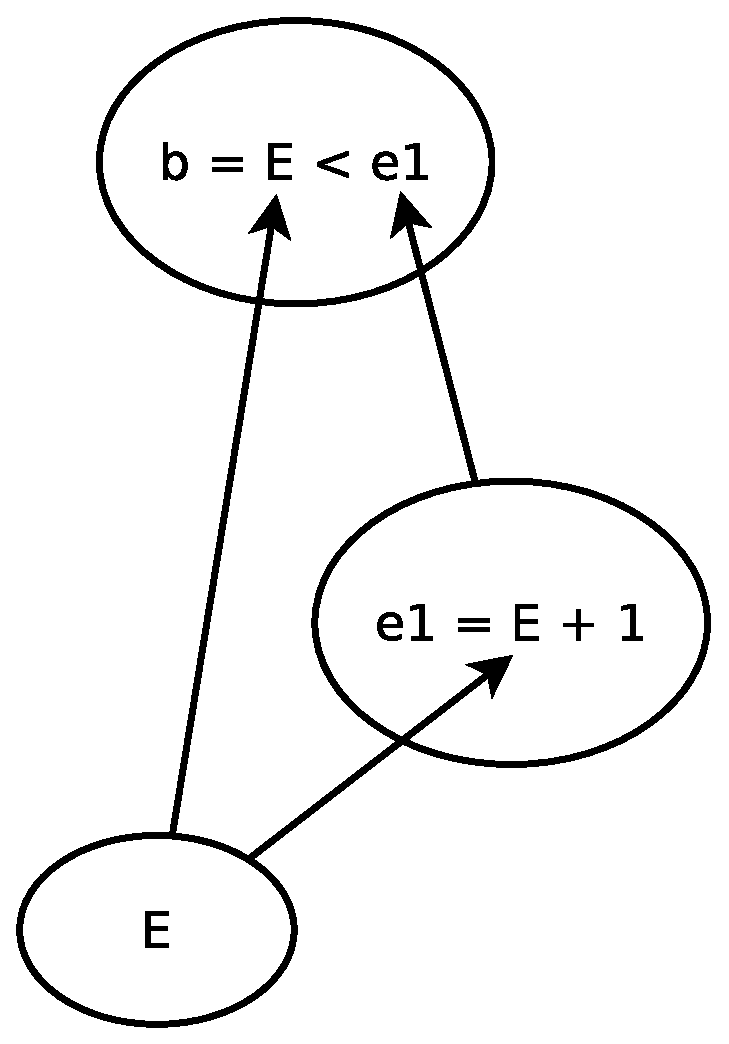
\includegraphics[width=\textwidth]{s}
\hspace{0.0cm}
\end{minipage}
%
\begin{minipage}[t]{0.10\linewidth}
\hspace{0.4cm}
\end{minipage}
\begin{minipage}[t]{0.55\linewidth}
\begin{lstlisting}[numbers=left,xleftmargin=0em]
input int E;
event int b, e1;
par/or do
  // b = E < E + 1
  loop do
    var int v1=0,v2=1;
    par/hor do
      v1 = await E;
    with
      v2 = await e1;
    end
    emit b => v1 < v2;
  end
with
  // s1 = s + 1
  loop do
    var int v = await E;
    emit e1 => v + 1;
  end
end
\end{lstlisting}
\end{minipage}
%\rule{8.4cm}{0.37pt}
\caption{ Glitch avoidance in \CEU with a \code{par/hor}.
\label{fig.glitch}
{\small
%TODO.
}
\label{lst.glitch}
}
\end{figure}

Mutual dependency is another known issue in dataflow languages, requiring the 
explicit placement of a specific delay operator to avoid runtime
cycles in some systems~\cite{frtime.embedding,luagravity.sblp}.
%
However, an explicit delay is somewhat \emph{ad hoc} because it splits an 
internal dependency problem across two reactions to the environment.
%
\CEU relies on the stack-based execution for internal events to avoid runtime 
cycles.
%
As an example, the program in Figure~\ref{lst.frp2} applies the temperature 
conversion formula between Celsius and Fahrenheit, so that whenever the value 
in one unit is set, the other is automatically recalculated (a problem proposed 
in~\cite{frp.survey}).
%
\begin{figure}[t]
%\rule{8.5cm}{0.37pt}
\begin{lstlisting}[numbers=left,xleftmargin=2em]
event int tc, tf;
par/or do
    loop do                // 1st trail
        var int v = await tc;
        emit tf => (9 * v / 5 + 32);
    end
with
    loop do                // 2nd trail
        var int v = await tf;
        emit tc => (5 * (v-32) / 9);
    end
with
    <...>                  // 3rd trail
    emit tc => 0;
end
\end{lstlisting}
\caption{ A dataflow program with mutual dependency.
\label{lst.frp2}
}
\end{figure}
%
We first define the \code{tc} and \code{tf} events to signal temperature 
changes.
Then, we create the 1st and 2nd trails to await for changes and mutually update 
the temperatures.
The third trail signals a temperature change and the program behaves as follows 
(with the stack in emphasis):
%
{\small
\begin{enumerate}
\setlength{\itemsep}{0pt}
\item 3rd trail signals \code{tc=>0} (line 14) and pauses.\\
    \emph{stack: [3rd]}
\item 1st trail awakes (line 4), signals \code{tf=>32} (line 5), and pauses.\\
    \emph{stack: [3rd,1st]}
\item 2nd trail awakes (line 9), signals \code{tc=>0} (line 10), and pauses.\\
    \emph{stack: [3rd,1st,2nd]}
\item no trails are awaiting \code{tc} (1st trail is paused at line 5, breaking 
    the cycle), so 2nd trail (on top of the stack) resumes, loops, and awaits 
\code{tf} again.\\
    \emph{stack: [3rd,1st]}
\item 1st trail resumes, loops, and awaits \code{tc} again (line 4).\\
    \emph{stack: [3rd]}
\item 3rd trail resumes with all dependencies resolved and terminates the 
    program.\\
    \emph{stack: []}
\end{enumerate}
}
%
As seen in step 4, the second \code{emit tc=>0} (line 10) is ignored by the 1st 
trail which is stacked in the reaction to the first \code{emit tc=>0} (line 
14).
%
This way, the stack-based execution for internal events can unambiguously 
express mutual dependencies.
%
%It also ensures that an \code{emit} that triggers nested dependencies only 
%resumes after the relationships are completely updated.
%
An actual application would run the dependency code in parallel and invoke
\code{await} and \code{emit} on the events \code{tc} and \code{tf}.

\begin{comment}
Again, the dataflow mechanism can be hidden with some syntactic sugar
 these exception mechanisms could be exposed in a higher level to developers.

The complexity of the solution is disproportionate to the problem it solves, 
but illustrates the circular dependency issue (a similar example appears in 
other references~\cite{frp.survey,frtime.embedding}).
The bottom line is that dataflow techniques permit that complex dependency 
patterns are handled internally, providing well-defined entry points to 
application programmers (i.e. they would be required to write only the 3rd and 
4th trails in the example).
- same semantics: no additional complexity
- additional syntax
- efficient
- limitation: only static

By definition, a Lustre program may not contain syntac-
tically cyclic definitions. The commercial Scade tool pro-
vides an option for an even stronger constraint that forbids an
output of a node to be fed back as an input without an inter-
operator. Users generally accept these constraints.
vening
The first constraint ensures that there is a static dependence
order between flows and allows a very simple generation of
sequential code (the scheduling is just topological sorting).
%\cite{rp.twenty}

DEPRECATING ODERSKY
In order to prevent reactives from observing
inconsistent data (also called glitches) during and between
propagation cycles, we keep the dependency graph topolog-
ically sorted.

EMBEDDING
However, they enforce a topological order, which guarantees the absence of 
glitches and makes the state at the end of each update cycle well-defined.

ROY
This implementation can give a
glitch, for example if the new value of x reaches the addition before the new result of
the multiplication. This gives a temporary result of 17, which is incorrect. Glitches
are a source of nondeterminism that the implementation must avoid, for example by
compile-time preprocessing (doing a topological sort of operations) or thread scheduling
constraints. Some languages that implement this paradigm are Yampa (embedded in
Haskell) [27] and FrTime (embedded in Scheme) [12].

Most reactive programming languages eliminate glitches by arranging expressions 
in a topologically sorted graph [Cooper and Krishnamurthi 2006]; [Meyerovich
et al. 2009]; [Maier et al. 2010], thus ensuring that an expression is always evaluated
after all its dependents have been evaluated.
Most recent reactive implementations achieve glitch avoidance in reactive programs
running on a single computer, but not in distributed reactive programs. Avoiding
glitches in a distributing setting is not straightforward because of network failures,
delays and lack of a global clock. This is a potential sweet spot for future research
on distributed reactive systems that provide glitch freedom. We further discuss dis-
tributed reactive programming as an open issue in Section 5.
Also, an efficient reactive implementation should avoid unnecessary recomputations
of values that do not change. Dependent computations need not be recomputed if the
value they depend on is updated to a new value that is the same as the previous
value. Taking the same example above, suppose the value of var1 that is initially 1, is
afterwards updated to the same value (i.e., 1). In such a case, the values for var2 and
var3 need not to be recomputed as the value of var1 remained unchanged.
\end{comment}

%\newpage
%\section{Implementation of \CEU}
%\subsection{Operational semantics}
%\textbf{Formalization}
\section{The semantics of C\'eu}
\label{sec.sem}

We present a formal semantics of \CEU focusing on the control aspects of the 
language, with a reduced syntax as follows:
%
%\begin{figure}[h]
%\rule{8.5cm}{0.37pt}
{\small
\begin{verbatim}
                          // primary expressions
  p ::= mem(id)           (any memory access to `id')
      | await(id)         (await event `id')
      | emit(id)          (emit event `id')
      | break             (loop escape)
                          // compound expressions
      | mem(id) ? p : p   (conditional)
      | p ; p             (sequence)
      | loop p            (repetition)
      | p and p           (par/and)
      | p or p            (par/or)
      | p hor q           (par/hor)
                          // derived by semantic rules
      | awaiting(id,n)    (awaiting `id' since seqno `n')
      | emitting(n)       (emitting on stack level `n')
      | p @ loop p        (unwinded loop)
\end{verbatim}
}%
%\caption{
    %Reduced syntax of \CEU.
%\label{lst.syntax}
%}
%\end{figure}
%
The $mem(id)$ primitive represents all accesses, assignments, and $C$ function 
calls that affect a memory location identified by $id$.
As the challenging parts of \CEU reside on its control structures, we are not 
concerned here with a precise semantics for side effects, but only with their 
occurrences in programs.
%In accordance with the zero-delay hypothesis of \CEU, $mem$ expressions are 
%considered to be atomic and instantaneous
%
The special notation $nop$ is used to represent an innocuous $mem$ expression 
(it can be though as a synonym for $mem(\epsilon)$, where $\epsilon$ is an 
unused identifier).
%
All other expressions map to their counterparts in the concrete language in 
TTT.
%
Note that $mem$ expressions cannot share identifiers with $await$/$emit$ 
expressions.

The core of our semantics is a relation that, given a sequence number $n$ 
identifying the current reaction chain, maps a program $p$ and a stack of 
events $S$ in a single step to a modified program and stack:
%
$$
\LL S, p \RR
    \xrightarrow[~~n~~]{}
\LL S', p' \RR
$$
%
where
%
\begin{align*}
S, S' &\in id^*
    &&(sequence~of~event~identifiers: [id_{top}, ..., id_1]) \\
p, p' &\in P
    && (as~described~in~the~syntax~above) \\
n     &\in \mathds{N}
    && (univocally~identifies~a~reaction~chain)
\end{align*}

At the beginning of a reaction chain, the stack is initialized with the special 
$\eta$ event and the occurring external event $ext$ ($S=[\eta,ext]$), but 
$emit$ expressions can push new events on top of it (we discuss how they are 
popped further).
%
The event $\eta$ is used as a special marker to check for pending \emph{hor} 
expressions before terminating the reaction.

We describe this relation with a set of \emph{small-step} structural semantics 
rules, which are built in such a way that at most one transition is possible at 
any time, resulting in deterministic reaction chains.
%
Figure~\ref{fig.sem} shows the transitions rules for the complete semantics of 
\CEU.

\begin{figure}
%
{ \setlength{\jot}{7pt}
\begin{align*}
\LL S,\1await(id) \RR &\ST
\LL S,\1awaiting(id,n) \RR
    & \rr{(await)}      \\
%%%
\LL id:S,\1awaiting(id,m) \RR &\ST
\LL id:S,\1nop \RR, \2m<n
    & \rr{(awaiting)}   \\
%%%
\LL S,\1emit(id) \RR &\ST
\LL id:S,\1emitting(|S|) \RR
    & \rr{(emit)}       \\
%%%
\LL S,\1emitting(|S|) \RR &\ST
\LL S,\1nop \RR
    & \rr{(emitting)}
\end{align*}
%}
}
%
%{ \setlength{\jot}{7pt}
{ %\normalsize
\begin{eqnarray*}
& \frac
    { \DS val(id,n) \neq 0 }
%   -----------------------------------------------------------
    { \DS \LL S, (mem(id)~?~p~:~q) \RR \ST
          \LL S, p \RR }
    & \rr{(if-true)}       \\
%%%
& \frac
    { \DS val(id,n) = 0 }
%   -----------------------------------------------------------
    { \DS \LL S, (mem(id)~?~p~:~q) \RR \ST
          \LL S, q \RR }
    & \rr{(if-false)}       \\
%%%
& \frac
    {\DS \LL S,p \RR \ST \LL S',p' \RR }
%   -----------------------------------------------------------
    {\DS \LL S, (p~;~q) \RR \ST \LL S', (p'~;~q) \RR }
    & \rr{(seq-adv)}        \\
%%%
& \LL S, (mem(id)~;~q) \RR \ST  \LL S, q \RR
    & \rr{(seq-nop)}        \\
%%%
& \LL S, (break~;~q) \RR \ST \LL S, break \RR
    & \rr{(seq-brk)}        \\
%\end{eqnarray*}
%}
%
%{ \setlength{\jot}{7pt}
%\begin{eqnarray*}
& \LL S, (loop~p) \RR \ST \LL S, (p~@~loop~p) \RR
    & \rr{(loop-expd)}       \\
%%%
& \frac
    {\DS \LL S,p \RR \ST \LL S',p' \RR }
% -----------------------------------------------------------
    {\DS \LL S, (p~@~loop~q) \RR \ST \LL S', (p'~@~loop~q) \RR }
    & \rr{(loop-adv)}    \\
%%%
& \LL S, (mem(id)~@~loop~p) \RR \ST \LL S, loop~p \RR
    & \rr{(loop-nop)}    \\
%%%
& \LL S, (break~@~loop~p) \RR \ST \LL S, nop \RR
    & \rr{(loop-brk)}       \\
%\end{eqnarray*}
%}
%
%{ \setlength{\jot}{7pt}
%\begin{eqnarray*}
& \frac
    {\DS \LL S,p \RR \ST \LL S',p' \RR }
%   -----------------------------------------------------------
    {\DS \LL S, (p~par~q) \RR \ST \LL S', (p'~par~q) \RR }
    & \rr{(par-adv1)}      \\
%%%
& \frac
    {\DS isBlocked(n,S,p) \1,\2 \LL S,q \RR \ST \LL S',q' \RR }
%   -----------------------------------------------------------
    {\DS \LL S, (p~par~q) \RR \ST \LL S', (p~par~q') \RR }
    & \rr{(par-adv2)}      \\
%%%
& \LL S, (mem(id)~and~q) \RR \ST \LL S, q \RR
    & \rr{(and-nop1)}   \\
%%%
& \LL S, (p~and~mem(id)) \RR \ST \LL S, p \RR
    & \rr{(and-nop2)}   \\
%%%
& \LL S, (break~and~q) \RR \ST \LL S, (clear(q)~;~break) \RR
    & \rr{(and-brk1)}   \\
%%%
& \frac
    {\DS isBlocked(n,S,p) }
%   -----------------------------------------------------------
    {\DS \LL S, (p~and~break) \RR \ST \LL S, (clear(p)~;~break) \RR }
    & \rr{(and-brk2)}   \\
%\end{eqnarray*}
%}
%
%{ \setlength{\jot}{7pt}
%\begin{eqnarray*}
%
%%%
& \frac
    {\DS \LL S,p \RR \ST \LL S',p' \RR }
%   -----------------------------------------------------------
    {\DS \LL S, (p~or~q) \RR \ST \LL S', (p'~or~q) \RR }
    & \rr{(or-adv1)}   \\
%%%
& \frac
    {\DS isBlocked(n,S,p) \1,\2 \LL S,q \RR \ST \LL S',q' \RR }
%   -----------------------------------------------------------
    {\DS \LL S (p~or~q) \RR \ST \LL S', (p~or~q') \RR }
    & \rr{(or-adv2)}   \\
%%%
& \LL S, (mem(id)~or~q) \RR \ST \LL S, clear(q) \RR
    & \rr{(or-nop1)}   \\
%%%
& \frac
    {\DS isBlocked(n,S,p) }
%   -----------------------------------------------------------
    {\DS \LL S, (p~or~mem(id)) \RR \ST \LL S, clear(p) \RR }
    & \rr{(or-nop2)}   \\
%%%
& \LL S, (break~or~q) \ST \LL S, (clear(q)~;~break) \RR
    & \rr{(or-brk1)}   \\
%%%
& \frac
    {\DS isBlocked(n,S,p) }
%   -----------------------------------------------------------
    {\DS \LL S, (p~or~break) \RR \ST \LL S, (clear(p)~;~break) \RR }
    & \rr{(or-brk2)}   \\
%%%
& \frac
    {\DS q \neq (a~hor~b) \1\vee\1 (a \neq nop \1\wedge\1 b \neq nop) }
%   -----------------------------------------------------------
    {\DS \LL [\eta], (nop~hor~q) \RR \ST \LL [\eta], nop \RR }
    & \rr{(hor-nop1)}   \\
%%%
& \frac
    {\DS p \neq (a~hor~b) \1\vee\1 (a \neq nop \1\wedge\1 b \neq nop) }
%   -----------------------------------------------------------
    {\DS \LL [\eta], (p~hor~nop) \RR \ST \LL [\eta], nop \RR }
    & \rr{(hor-nop2)}
%
\end{eqnarray*}
}
%
\caption{ The semantics of \CEU.
\label{fig.sem}
}
\end{figure}

An $await$ is simply transformed into an $awaiting$ that remembers the current 
external sequence number $n$ (rule \textbf{await}).
An $awaiting$ can only transit to a $nop$ (rule \textbf{awaiting}) if its 
referred event $id$ matches the top of the stack and its sequence number is 
smaller than the current one ($m<n$).
%
%Remember that in \CEU, the \code{await} statement returns the value associated 
%with the corresponding event: the yielded $mem$ represents the operation to 
%query that value.
%
An $emit$ transits to an $emitting$ holding the current stack level ($|S|$ 
stands for the stack length), and pushing the referred event on the stack (in 
rule \textbf{emit}).
With the new stack level $|S|+1$, the $emitting(|S|)$ itself cannot transit, as 
rule \textbf{emitting} expects its parameter to match the current stack level.
This trick provides the desired stack-based semantics for internal events.

Proceeding to compound expressions, the rules for conditionals and sequences 
are straightforward.
%
Given that our semantics focuses on control, rules \textbf{if-true} and 
\textbf{if-false} are the only to query $mem$ expressions.
%
The ``magical'' function $val$ receives the memory identifier and current 
reaction sequence number, returning the current memory value.
%
Although the value is arbitrary, it is unique in a reaction chain, because a 
given expression can execute only once within it (remember that $loops$ must 
contain $awaits$ which, from rule \textbf{await}, cannot awake in the same 
reaction they are reached).
%For all other rules, we omit these values (e.g., \textbf{seq-nop}).

The rules for loops are analogous to sequences, but use \code{`@'} as 
separators to properly bind breaks to their enclosing loops.
%
When a program first encounters a $loop$, it first expands its body in sequence 
with itself (rule \textbf{loop-expd}).
Rules \textbf{loop-adv} and \textbf{loop-nop} are similar to rules 
\textbf{seq-adv} and \textbf{seq-nop}, advancing the loop until they reach a 
$mem(id)$.
However, what follows the loop is the loop itself (rule \textbf{loop-nop}).
Note that if we used \code{`;'} as a separator in loops, rules 
\textbf{loop-brk} and \textbf{seq-brk} would conflict.
%
Rule \textbf{loop-brk} escapes the enclosing loop, transforming everything into 
a $nop$.

The rules with the \rr{par} prefix are valid for all $and$/$or$/$hor$ 
compositions (substituting the $par$ in the rules for each of them).
%
The rules \rr{par-adv1} and \rr{par-adv2} force the transitions on the left 
branch $p$ to occur before transitions on the right branch $q$.
%
The deterministic behavior of the semantics relies on the \emph{isBlocked} 
predicate, defined in Figure~\ref{fig.isBlocked} and used in rule 
\textbf{and-adv2}, requiring the left branch $p$ to be blocked in order to 
allow the right transition from $q$ to $q'$.
%
An expression becomes blocked when all of its trails in parallel hang in 
$awaiting$ and $emitting$ expressions.

\begin{figure}[t]
{\small
\begin{align*}
  isBlocked(n,a:S, awaiting(b,m)) &= (a \neq b \1\vee\1 m = n)   \\
  isBlocked(n,S, emitting(s))    &= (|S| \neq s)                     \\
  isBlocked(n,S, (p~;~q))        &= isBlocked(n,S,p)             \\
  isBlocked(n,S, (p~@~loop~q))   &= isBlocked(n,S,p)             \\
  isBlocked(n,S, (p~and~q))      &= isBlocked(n,S,p)~\wedge
                               \\&~~~~isBlocked(n,S,q)             \\
  isBlocked(n,S, (p~or~q))       &= isBlocked(n,S,p)~\wedge
                               \\&~~~~isBlocked(n,S,q)             \\
  isBlocked(n,S, \_)             &= false \2  (mem,await,      \\
                                  &    \5\5\5\2 emit,break,if,loop)   %\\
\end{align*}
}%
%\rule{14cm}{0.37pt}
\caption{
The recursive predicate $isBlocked$.
% is true only if all branches in parallel are hanged in $awaiting$ or 
%$emitting$ expressions that cannot transit.
\label{fig.isBlocked}
}
\end{figure}

The rules \rr{par-brk1} and \rr{par-brk2} deal with a $break$ in each of the 
parallel sides.
A $break$ should terminate the whole composition in order to escape the 
innermost loop (\emph{aborting} the other side).

The difference betwen the three parallel compositions consists in how to deal 
with one of the sides terminating with a $nop$.
%
For an $and$ composition, if one of the sides terminates, the composition is 
simply substituted by the other side, as both sides are required to terminate 
(rules \rr{and-nop1} and \rr{and-nop2}).
%
For a parallel $or$, reaching a $nop$ in either of the sides should 
immediatelly terminate the composition (rules \rr{or-nop1} and \rr{or-nop2}).
%Note that rule \rr{xor-nop1} strongly aborts trail $q$ as soon as $p$ reaches 
%a $nop$
%
However, for a parallel $hor$ it is not enough that one of the sides reaches a 
$nop$, as the other should still be allowed to react.
The rules \rr{hor-nop1} and \rr{hor-nop2} ensure, first, that a composition 
rejoins only after no transitions are possible in either sides, and second, 
that rejoins happen from inside out, i.e., that nested compositions rejoin 
before outer compositions.
The first condition is achieved by only allowing transitions with $s=0$, when 
the program is guaranteed to be blocked.
For the second condition, we check if a nested $hor$ is also pending, forcing 
it to transit before (via rules \rr{par-adv1} or \rr{par-adv2}).

A reaction chain eventually blocks in $awaiting$ and $emitting$ expressions in 
parallel trails.
%
If all trails hangs only in $awaiting$ expressions, it means that the program 
cannot advance in the current reaction chain.
%
However, $emitting$ expressions should resume their continuations of previous 
$emit$ in the ongoing reaction, they are just hanged in lower stack indexes 
(see rule \textbf{emit}).
%
Therefore, we define another relation that behaves as the previous if the 
program is not blocked, and, otherwise, pops the stack:
%
$$
\frac
    { \DS \LL S,p \RR \ST                   \LL S',p' \RR }
%   -----------------------------------------------------------
    {     \LL S,p \RR \xRightarrow[~~n~~]{} \LL S',p' \RR }
%
\5\5\5
%
\frac
    { \DS isBlocked(n,\1s:S,\1p) }
%   -----------------------------------------------------------
    { \LL s:S,p \RR \xRightarrow[~~n~~]{} \LL S,p \RR }
$$
%
To describe a \emph{reaction chain} in \CEU, i.e., how a program behaves in 
reaction to a single external event, we use the reflexive transitive closure of 
this relation:
%
$$
    \LL S,p \RR \xRightarrow[~~n~~]{*} \LL S',p' \RR
$$
%
Finally, to describe the complete execution of a program, we need multiple 
``invocations'' of reaction chains, incrementing the sequence number:
%
\begin{align*}
\LL [\eta,e1], p \RR
    & \xRightarrow[~~1~~]{*}
\LL [  ], p' \RR
\\
\LL [\eta,e2], p' \RR
    & \xRightarrow[~~2~~]{*}
\LL [  ], p'' \RR
\\
& ...
\end{align*}
%
Each invocation starts with an external event at the top of the stack and 
finishes with a modified program and an empty stack.
After each invocation, the sequence number is incremented.

%\newpage
\section{Related work}
\label{sec.related}

With respect to control-based languages for embedded systems, the emerging area 
of Wireless Sensor Networks produced a number of synchronous alternatives to 
low-level event-driven 
systems~\cite{wsn.protothreads,wsn.sol,wsn.osm,wsn.tinythreads}.
%
Some offer predictable and lightweight
multi-threading~\cite{wsn.protothreads,wsn.tinythreads} with shared-memory 
concurrency, but lack thread composition and abortion (as described in 
Section~\ref{sec.ceu.abortion}).
They also do not provide first-class events or a powerful broadcast mechanism, 
limiting their control mechanisms.
%
OSM~\cite{wsn.osm} provides parallel state machines with a formal and mature 
synchronous model, with (equivalent) support to thread composition and 
abortion.
However, although machines can share memory, the execution order for operations 
among them is non-deterministic.
Also, describing sequential code across reactions is not straightforward with 
state machines~\cite{wsn.osm} (in comparison to \CEU's \code{await} statement).
%
Another Esterel-based language for constrained systems~\cite{wsn.sol} made 
similar design decisions to ours, handling a single external event at a time, 
and relying on a deterministic scheduler for safe memory sharing.

\emph{Functional Reactive Programming (FRP)} adapts modern functional languages 
to the reactive dataflow style~\cite{frp.principles}.
In particular, Flask~\cite{wsn.flask} shows that dataflow languages can also 
target constrained systems.
%
\CEU borrows some ideas from an FRP implementation \cite{frtime.embedding}, 
such as a push-driven evaluation and glitch prevention.
However, dataflow in \CEU is less abstract in comparison to FRP, and limited to 
static relationships only.

\begin{comment}
SHIM is an asynchronous language that enforces synchronous communications among 
processes, providing a deterministic execution model.
SHIM distinguishes from typical asynchronous languages given that
The use of point-to-point communication, typical in CSP-like 
languages~\cite{async.csp}, leads to a different programming mindset.
No shared-memory
no hierarchies (e.g., \code{par/or} compositions)

However, as far as we know, \CEU is the first language to provide a stack-based 
execution for internal events.
The intro
The stack-based policy for internal events is also...
%
None of these systems offer a construct equivalent to \CEU's \code{par/hor}, 
and we believe that they cannot describe data dependency reliably.
%
However, embedded systems are typically characterized by control-intensive 
applications, where programs have to deal with low-level I/O and handle 
explicit state.
In this context, dataflow programming does not provide proper abstractions, 
being more suitable for data-intensive applications.

\end{comment}

\section{Conclusion}
\label{sec.conclusion}

As a descendant of Esterel, \CEU achieves a high degree of reliability for 
embedded systems, while also embracing practical aspects, such as
shared-memory concurrency, and advanced control-flow mechanisms.
%
\CEU introduces a stack-based execution policy for internal events, expanding 
its expressiveness, such as for describing exceptions and dataflow programming 
without dedicated primitives.
%
Nonetheless, the language is still simple and all control details (e.g. 
deterministic execution, stack-based internal events, trail abortion) can be 
described with a compact formal semantics.

As far as we know, \CEU is the first language to reconcile the control and 
dataflow reactive styles.

\begin{comment}
We consider that providing safe shared-memory concurrency is a fundamental 
design choice of \CEU, given that low-level I/O is indispensable in the context 
of embedded systems (e.g. interfacing with sensors and actuators).

Embedded systems are still predominantly developed in the ``bare metal'', 
regardless of existing alternatives, probably due to the flexibility and 
popularity of $C$.
We believe that \CEU is an attractive alternative, given its unrestricted 
access to $C$ and rich set of concurrent control primitives (e.g., parallel 
compositions and internal events).
Limited but safer subroutines
\end{comment}

\bibliographystyle{abbrv}
\bibliography{other,my}

\end{document}
